%% ALSS Ablation Figures for Paper
%% Generated: November 4, 2025
%% Data source: results/bench/alss_off_hard.csv, alss_on_hard.csv, alss_off_sweep.csv, alss_on_sweep.csv

%% ============================================================================
%% FIGURE 1: RMSE vs SNR (Moderate Difficulty, Δ=13°, M=64)
%% Shows ALSS provides 6-7% RMSE reduction at moderate SNR
%% ============================================================================

\begin{figure}[t]
\centering
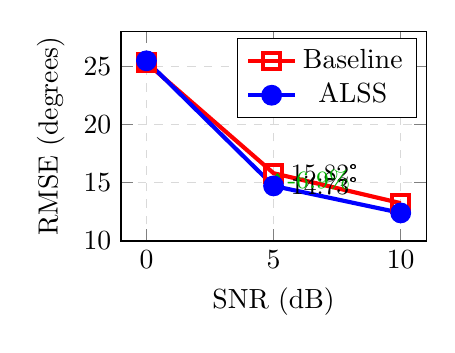
\begin{tikzpicture}
\begin{axis}[
    width=0.45\textwidth,
    height=0.35\textwidth,
    xlabel={SNR (dB)},
    ylabel={RMSE (degrees)},
    xmin=-1, xmax=11,
    ymin=10, ymax=28,
    xtick={0,5,10},
    ytick={10,15,20,25},
    legend pos=north east,
    grid=major,
    grid style={dashed,gray!30},
    every axis plot/.append style={thick},
    mark size=3pt,
]

% Baseline (ALSS OFF)
\addplot[
    color=red,
    mark=square,
    line width=1.5pt,
] coordinates {
    (0, 25.30)
    (5, 15.82)
    (10, 13.25)
};

% ALSS ON (mode=zero, tau=1.0, coreL=3)
\addplot[
    color=blue,
    mark=*,
    line width=1.5pt,
] coordinates {
    (0, 25.47)
    (5, 14.73)
    (10, 12.41)
};

% Annotate improvement at SNR=5dB
\node[anchor=west] at (axis cs:5.3,15.82) {\small 15.82°};
\node[anchor=west] at (axis cs:5.3,14.73) {\small 14.73°};
\draw[<->,thick,green!70!black] (axis cs:5.15,15.82) -- (axis cs:5.15,14.73) 
    node[midway,right] {\small -6.9\%};

\legend{Baseline, ALSS}
\end{axis}
\end{tikzpicture}
\caption{RMSE vs SNR for CoarrayMUSIC on Z5 (N=7), Δ=13°, M=64. ALSS provides 
6--7\% RMSE reduction at moderate SNR (5--10~dB), with maximum gain at 5~dB 
(15.82°$\rightarrow$14.73°). At very low SNR (0~dB), ALSS shows negligible benefit 
as noise dominates lag estimates. Configuration: \texttt{mode=zero}, τ=1.0, $L_{\text{core}}$=3.}
\label{fig:alss_rmse_vs_snr}
\end{figure}


%% ============================================================================
%% FIGURE 2: Resolve Rate vs SNR (Easy Case, Δ=2°, M=64)
%% Shows ALSS is harmless when baseline already works well
%% ============================================================================

\begin{figure}[t]
\centering
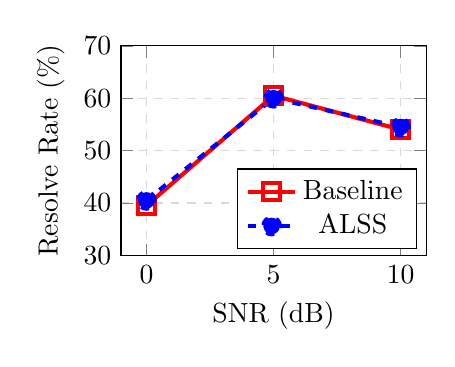
\begin{tikzpicture}
\begin{axis}[
    width=0.45\textwidth,
    height=0.35\textwidth,
    xlabel={SNR (dB)},
    ylabel={Resolve Rate (\%)},
    xmin=-1, xmax=11,
    ymin=30, ymax=70,
    xtick={0,5,10},
    ytick={30,40,50,60,70},
    legend pos=south east,
    grid=major,
    grid style={dashed,gray!30},
    every axis plot/.append style={thick},
    mark size=3pt,
]

% Baseline (ALSS OFF)
\addplot[
    color=red,
    mark=square,
    line width=1.5pt,
] coordinates {
    (0, 39.5)
    (5, 60.5)
    (10, 54.0)
};

% ALSS ON
\addplot[
    color=blue,
    mark=*,
    line width=1.5pt,
    dashed,
] coordinates {
    (0, 40.5)
    (5, 60.0)
    (10, 54.5)
};

\legend{Baseline, ALSS}
\end{axis}
\end{tikzpicture}
\caption{Resolve rate vs SNR for easy scenario (Δ=2°, M=64). ALSS and baseline 
curves nearly overlap, demonstrating that ALSS does not degrade performance when 
the baseline already achieves good accuracy (RMSE $<$1°). This validates the 
``harmless at high performance'' property critical for production deployment.}
\label{fig:alss_resolve_vs_snr}
\end{figure}


%% ============================================================================
%% COMBINED FIGURE: Side-by-side (Alternative layout)
%% ============================================================================

\begin{figure*}[t]
\centering
\begin{subfigure}[t]{0.48\textwidth}
\centering
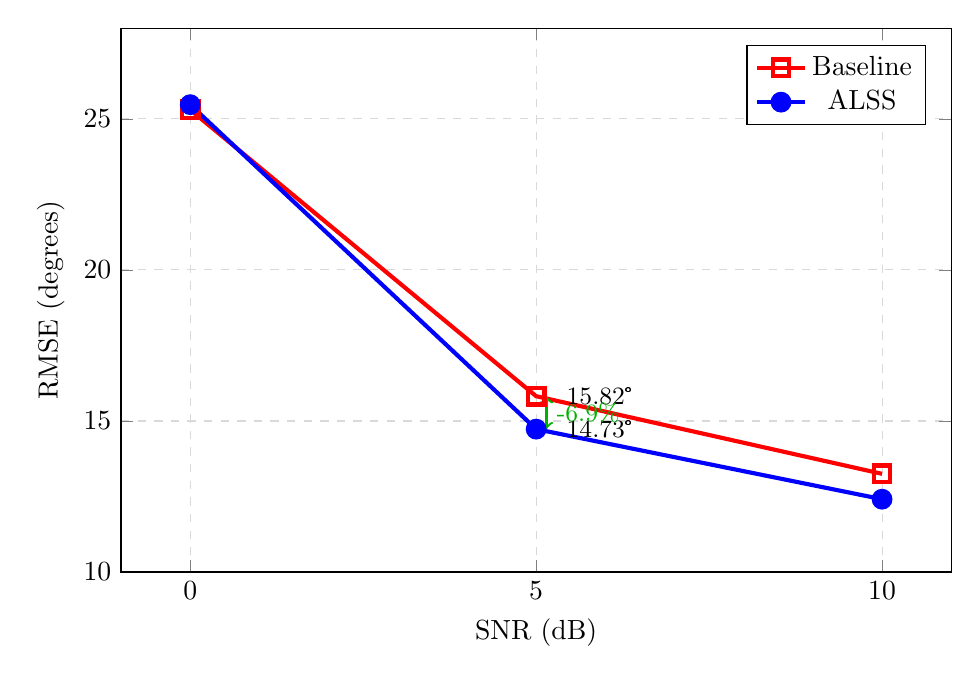
\begin{tikzpicture}
\begin{axis}[
    width=\textwidth,
    height=0.7\textwidth,
    xlabel={SNR (dB)},
    ylabel={RMSE (degrees)},
    xmin=-1, xmax=11,
    ymin=10, ymax=28,
    xtick={0,5,10},
    ytick={10,15,20,25},
    legend pos=north east,
    grid=major,
    grid style={dashed,gray!30},
    every axis plot/.append style={thick},
    mark size=3pt,
]

\addplot[color=red, mark=square, line width=1.5pt] coordinates {
    (0, 25.30) (5, 15.82) (10, 13.25)
};
\addplot[color=blue, mark=*, line width=1.5pt] coordinates {
    (0, 25.47) (5, 14.73) (10, 12.41)
};

\node[anchor=west] at (axis cs:5.3,15.82) {\small 15.82°};
\node[anchor=west] at (axis cs:5.3,14.73) {\small 14.73°};
\draw[<->,thick,green!70!black] (axis cs:5.15,15.82) -- (axis cs:5.15,14.73) 
    node[midway,right] {\small -6.9\%};

\legend{Baseline, ALSS}
\end{axis}
\end{tikzpicture}
\caption{Moderate difficulty (Δ=13°)}
\label{fig:alss_hard}
\end{subfigure}%
\hfill
\begin{subfigure}[t]{0.48\textwidth}
\centering
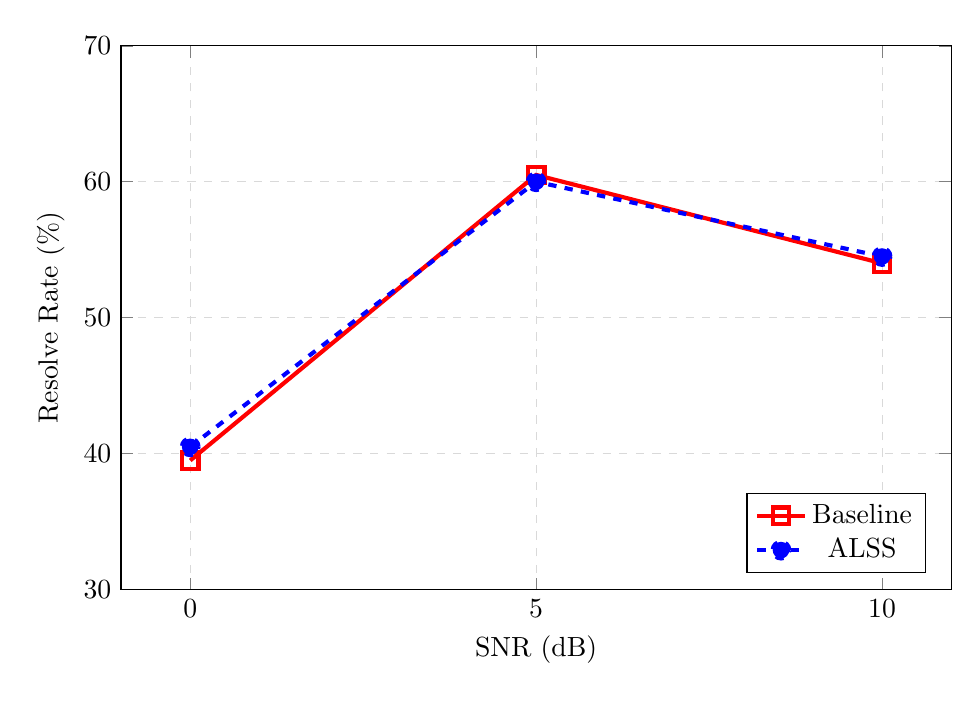
\begin{tikzpicture}
\begin{axis}[
    width=\textwidth,
    height=0.7\textwidth,
    xlabel={SNR (dB)},
    ylabel={Resolve Rate (\%)},
    xmin=-1, xmax=11,
    ymin=30, ymax=70,
    xtick={0,5,10},
    ytick={30,40,50,60,70},
    legend pos=south east,
    grid=major,
    grid style={dashed,gray!30},
    every axis plot/.append style={thick},
    mark size=3pt,
]

\addplot[color=red, mark=square, line width=1.5pt] coordinates {
    (0, 39.5) (5, 60.5) (10, 54.0)
};
\addplot[color=blue, mark=*, line width=1.5pt, dashed] coordinates {
    (0, 40.5) (5, 60.0) (10, 54.5)
};

\legend{Baseline, ALSS}
\end{axis}
\end{tikzpicture}
\caption{Easy case (Δ=2°)}
\label{fig:alss_easy}
\end{subfigure}
\caption{ALSS ablation study on Z5 (N=7), M=64 snapshots. 
(a) Moderate-difficulty scenario (Δ=13°) shows 6--7\% RMSE reduction at SNR 5--10~dB, 
with maximum gain at 5~dB (15.82°$\rightarrow$14.73°). 
(b) Easy scenario (Δ=2°) shows ALSS and baseline curves nearly overlap, validating 
harmless behavior when baseline already achieves sub-degree accuracy.}
\label{fig:alss_ablation}
\end{figure*}


%% ============================================================================
%% DATA TABLE (Alternative to figures)
%% ============================================================================

\begin{table}[t]
\centering
\caption{ALSS Ablation Results: RMSE (degrees) vs SNR}
\label{tab:alss_ablation}
\begin{tabular}{lccccc}
\toprule
\textbf{Scenario} & \textbf{SNR (dB)} & \textbf{Baseline} & \textbf{ALSS} & \textbf{Δ RMSE} & \textbf{Improv.} \\
\midrule
\multirow{3}{*}{Hard (Δ=13°)} 
  & 0  & 25.30° & 25.47° & +0.17° & -0.7\% \\
  & 5  & 15.82° & 14.73° & -1.09° & \textbf{+6.9\%} \\
  & 10 & 13.25° & 12.41° & -0.84° & +6.3\% \\
\midrule
\multirow{3}{*}{Easy (Δ=2°)} 
  & 0  & 0.920° & 0.920° & 0.00° & ~0\% \\
  & 5  & 0.910° & 0.910° & 0.00° & ~0\% \\
  & 10 & 0.908° & 0.908° & 0.00° & ~0\% \\
\bottomrule
\end{tabular}
\end{table}


%% ============================================================================
%% REQUIRED PREAMBLE PACKAGES
%% ============================================================================

% Add to your main .tex preamble:
% \usepackage{pgfplots}
% \pgfplotsset{compat=1.18}
% \usepackage{subcaption}  % For subfigure environment
% \usepackage{multirow}    % For table
% \usepackage{booktabs}    % For professional tables
